\chapter{Los rayos cósmicos}

\section{¿Qué son los rayos cósmicos?}

Los rayos cósmicos son núcleos ionizados mediante procesos de aceleración que viajan a través de la Vía Láctea, incluyendo el sistema solar. Se producen en estrellas, remanentes de supernovas, núcleos activos de galaxias y otros objetos astrofísicos. La composición de los rayos cósmicos es de aprox 93\% de protones, 6.3\% de partículas alfa y 0.7\% son núcleos de elementos más pesados. La pregunta fundamental es, ¿dónde se originan? y en particular, ¿como es que son aceleradas a tan altas energías?. La respuesta  a la pregunta del origen de los rayos cosmicos todavía no es totalmente conocido. Es claro, sin embargo, que casi todos ellos vienen desde fuera del sistema solar, pero desde dentro de la galaxia\cite{thomas}.\\

Se denominan rayos cósmicos primarios a las partículas que inciden en la atmósfera terrestre procedentes del espacio, compuestos principalmente de protones y partículas alfa. Al interactuar con un núcleo atmosférico producen una cascada de partículas compuesta por rayos $\gamma$, electrones, muones,etc, que son llamados rayos cósmicos secundarios\cite{spatium}.\\

El \emph{espectro de energía} de la radiación cósmica primaria describe cómo están distribuidas con respecto a la energía. En la Figura \ref{espectro}

\begin{figure}[H]
  \centering
    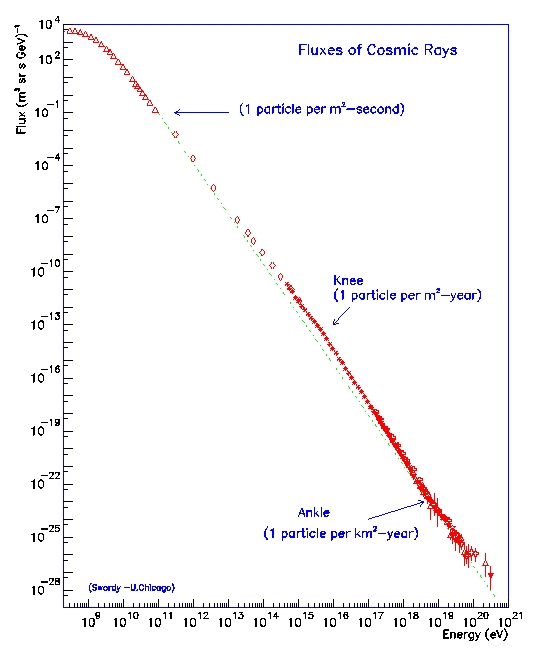
\includegraphics[scale=0.60]{Capitulo1/figs/esp.jpg}      %Ruta completa de la imagen, porque se compila desde el archivo tesis.tex
  \caption{Espectro de energía de rayos cósmicos.}            %Pie de imagen
  \label{espectro}                            %nombre de referencia
\end{figure}

Existe un gran número de mediciones y estudios del sector del
espectro con energías menores al tobillo; la existencia de la rodilla
está aún incompletamente explicada. Para energías mayores al tobillo
los rayos cósmicos ya no pueden ser confinados por el campo
magnético de la Vía Láctea y provienen de todas las direcciones por
igual. Esto indica que estos rayos cósmicos proceden de fuera de la
Galaxia. Además, las mediciones del grupo experimental Fly's Eye
sugieren que los rayos bajo el tobillo son principalmente núcleos de
átomos pesados(mayormente Fe), mientras que los eventos sobre el
tobillo son exclusivamente protones y neutrones. Esto es consistente
con la hipótesis de que los rayos supra-tobillos son extragalácticos, ya
que los núcleos pesados con energías superiores a 4x1018 eV no
podrían sobrevivir un viaje extragaláctico debido al roce con el Fondo
de Radiación Cósmica (FRC), mecanismo que se describirá más
adelante.



La Heliosfera es responsable de afectar a las partículas con energías que van desde los 109 eV a los 1015 eV, en la región del espectro conocida como ``rodilla", por debajo de esta zona, los RC galácticos son la contribución dominante. Las partículas con energías de \~1015-1017 eV son probablemente aceleradas por mecanismos de choques rápidos como los remanentes de supernovas.
Las partículas con energías superiores son llamadas “de ultra alta energía”, poseen radios de giro comparables con el radio de nuestra galaxia, son muy poco abundantes en comparación a los RC galácticos y su fuente aún no está plenamente confirmada, debido a esto, a menudo se les considera RC extra-galácticos. Alrededor de 1020 eV, el espectro comienza a aplanarse de nuevo, formando la región conocida como ``tobillo".

Durante muchos años se ha observado que la intensidad de los rayos cósmicos medida en la Tierra experimenta variaciones periódicas en función a las emisiones de la actividad del Sol, es decir, estas variaciones son producidas por la \emph{modulación solar}\cite{grieder}. La actividad solar modula el flujo de rayos cósmicos detectados en tierra. Entre las variaciones observadas en la radiación cósmica y que son influenciadas por el Sol se encuentran:

\begin{enumerate}[a)]
 \item \emph{La variación de 11 años}
 \item \emph{El decrecimiento Forbush}
 \item \emph{La variación diurna}
 \end{enumerate}

 
La \emph{variación de 11 años} está sujeta a una variación periódica debida al ciclo solar promedio de 11 años. Existe una anti-correlación entre los rayos cósmicos detectados y el número de manchas solares. Como el número de manchas solares es un indicador de la actividad solar, a mayor número de manchas, mayor actividad y emisiones en el Sol. Las emisiones de la actividad del Sol permean todo el Sistema Solar con líneas de campo magnético, las cuales desvían a los rayos cósmicos que ingresan. Cuando el Sol se encuentra con baja actividad, las emisiones son menos intensas y permiten que el flujo de rayos cósmicos galácticos se incremente. Por lo tanto, a mínimo número de manchas, menor cantidad de emisiones solares y mayor el flujo de rayos cósmicos detectados, con un retardo de aproximadamente 1 o 2 años\cite{stanev}. En la figura \ref{sunspot} se puede ver la anti-correlación entre el número de manchas solares observados por Solar Influences Data Analysis Center (SIDC)  y las cuentas del monitor de neutrones de Oulu.\\ 

El \emph{decrecimiento Forbush}, llamado así en honor al físico estadounidense Scott E. Forbush, es el decrecimiento repentino de la intensidad de la radiación cósmica hasta en un 10\% y ocasionalmente 20 o 30\% en el lapso de unas cuantas horas. Una vez que la intensidad ha llegado a un mínimo empieza a recuperarse gradualmente, lo cual puede durar varias horas, días o incluso semanas.\\

\begin{figure}[H]
\centering
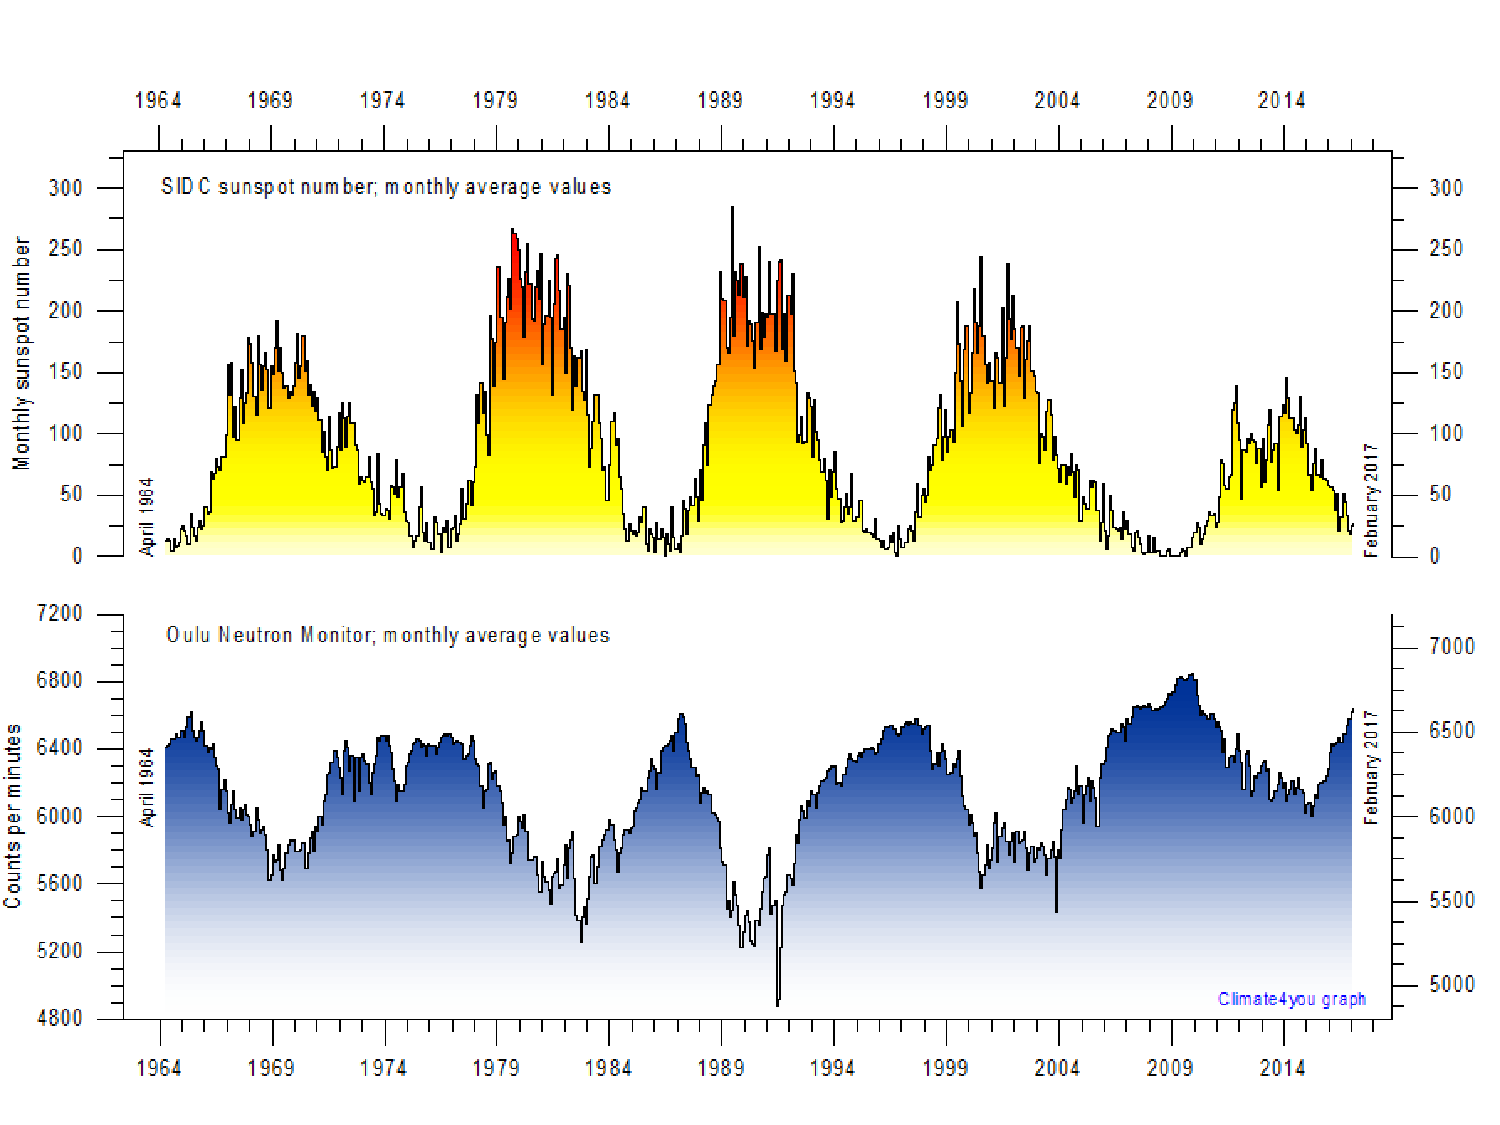
\includegraphics[scale=0.50]{Capitulo1/figs/cr_vs_sunspots.pdf}
\caption{Observaciones mensuales del número manchas solares (Solar Influences Data Analysis Center (SIDC)) desde abril de 1964, y medias mensuales de las cuentas del monitor de neutrones de Oulu (Finlandia), ajustados por presión barométrica y eficiencia. Actualización: 1 de marzo de 2017.}
\label{sunspot} 
\end{figure}
 
Aún se estudian los mecanismos y procesos de generación de los decrecimientos Forbush y se sabe que son un efecto de las líneas de campo magnético asociadas con las emisiones solares. En el momento que ocurre una ráfaga solar o una eyección de masa coronal de una región activa del Sol, la nube de plasma eyectada puede tener una velocidad más alta que el viento solar normal, lo cual produce una discontinuidad brusca conocida como \emph{onda de choque}. La onda de choque forma un ``contenedor" magnético con una intensidad de campo relativamente alta. Si la Tierra se encuentra dentro de este contenedor, la radiación cósmica es desviada en función a su energía y no ingresa a la atmósfera; a medida que esta onda se aleja, menos será la influencia sobre las partículas\cite{grieder,mensajeros}. En la figura \ref{forbush} se muestra un decrecimiento forbush detectado por el monitor de neutrones del Observatorio de Rayos Cósmicos de la Ciudad de México.\\

\begin{figure}[H]
\centering
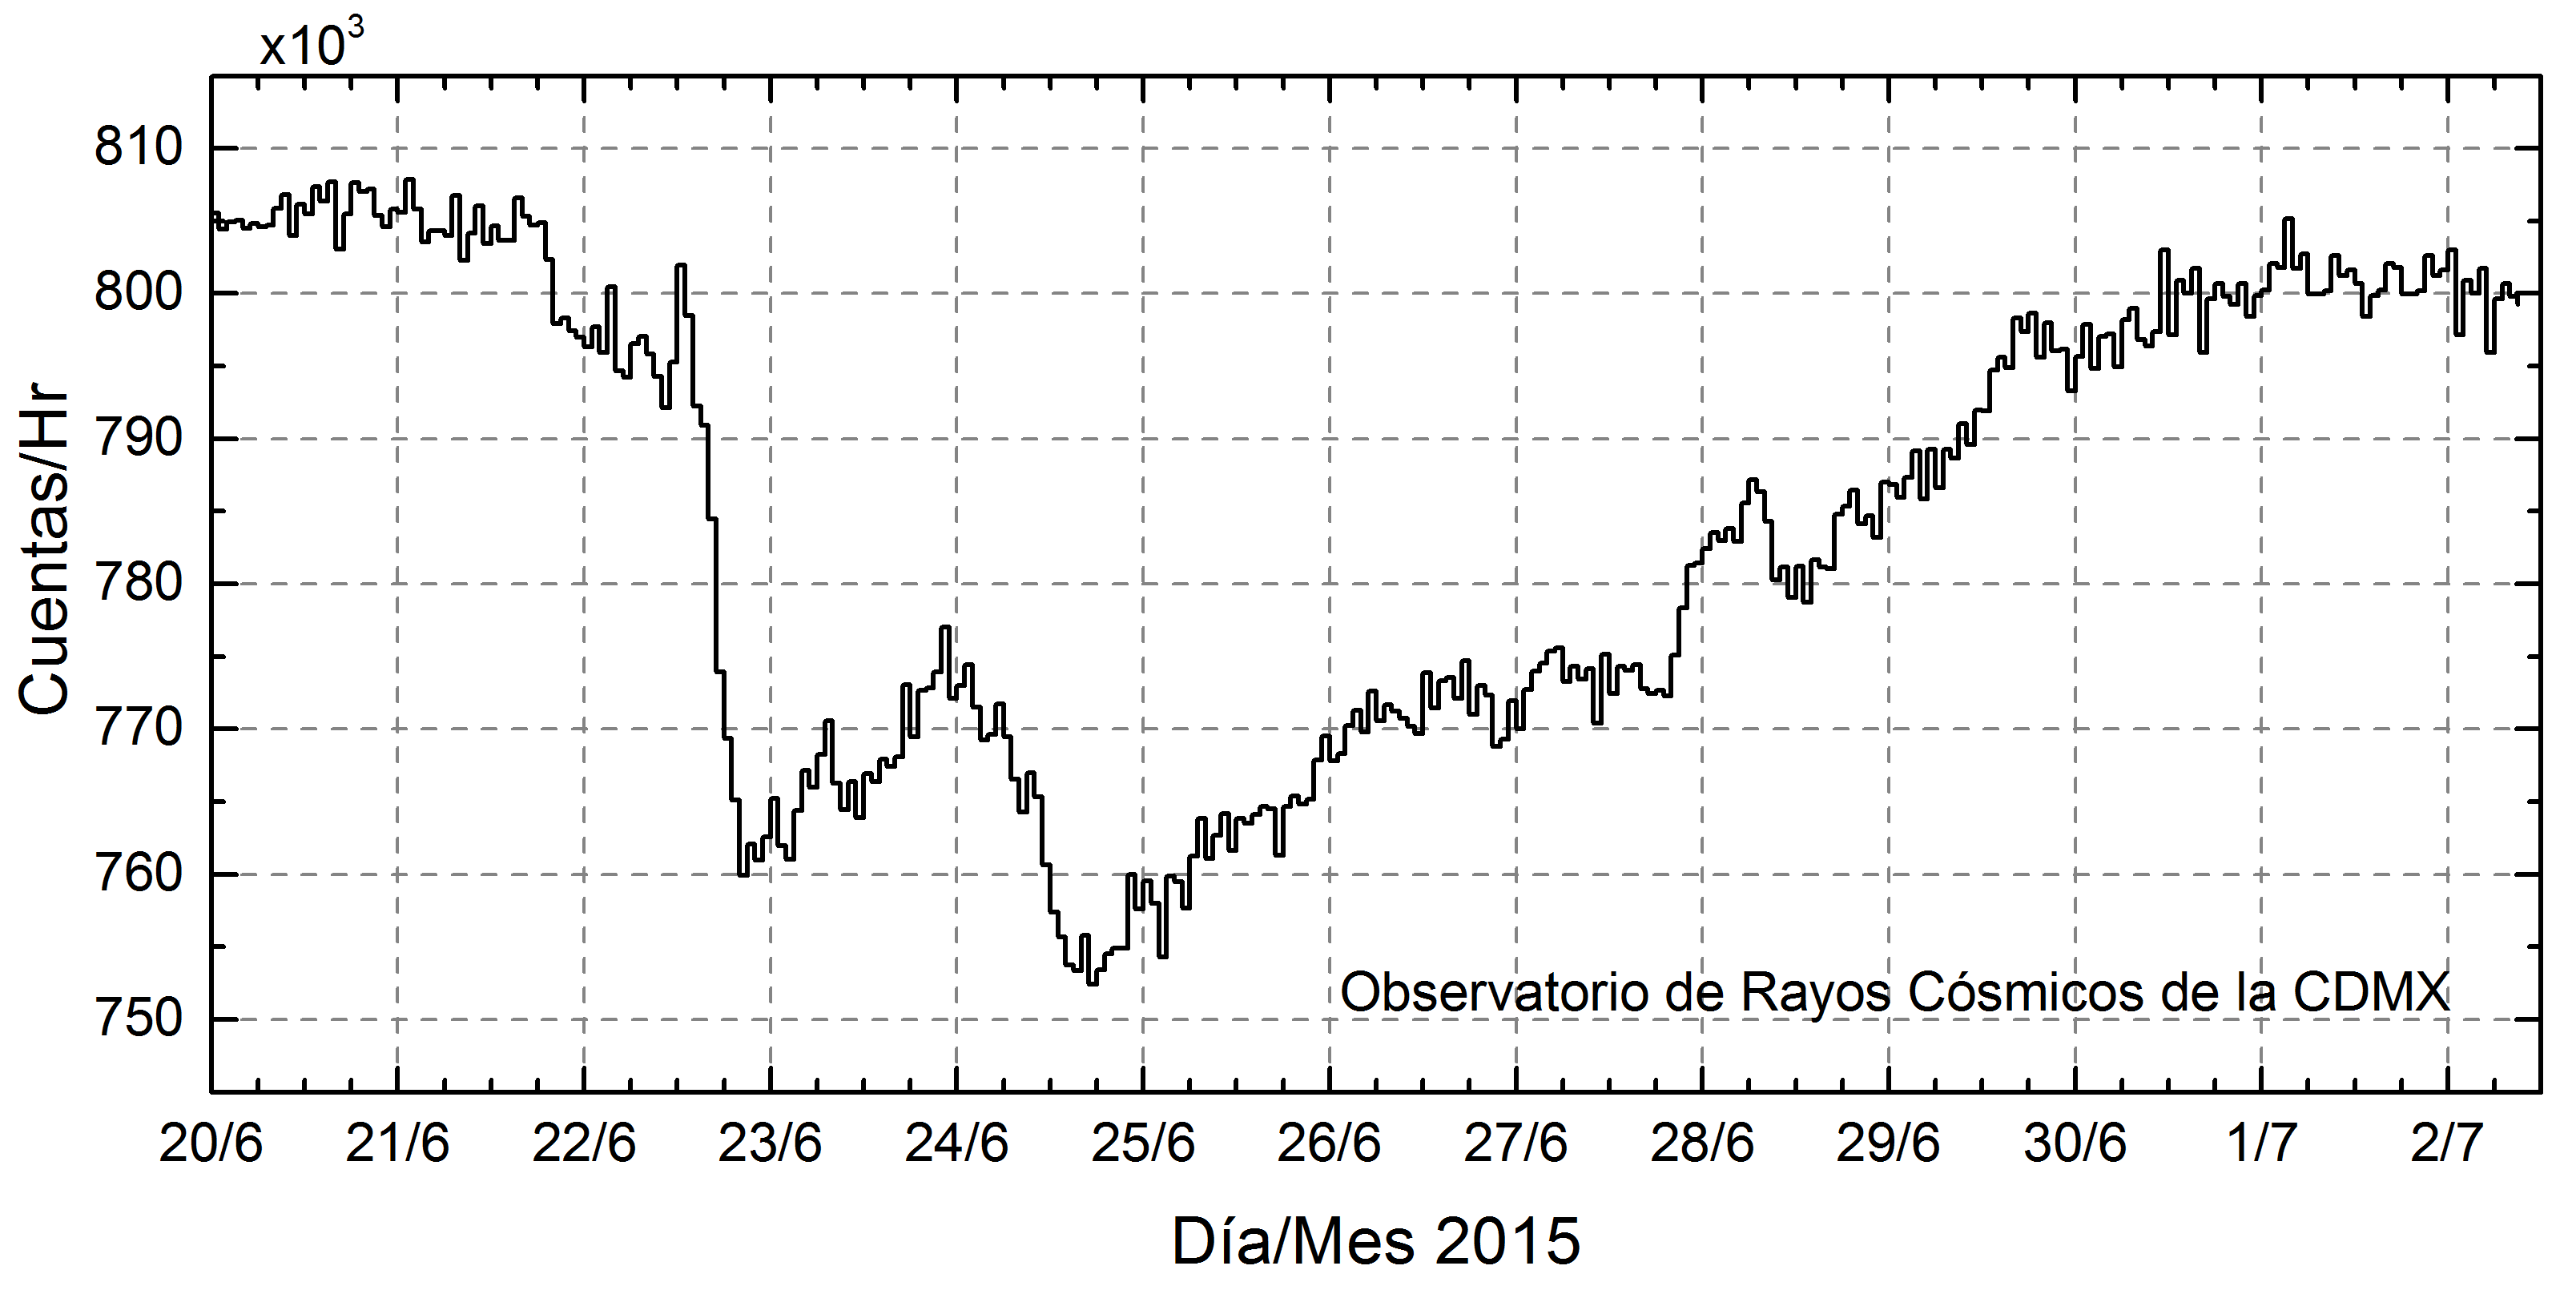
\includegraphics[scale=0.50]{Capitulo1/figs/Decrecimiento_Forbush.png}
\caption{Decrecimiento Forbush detectado por  el monitor de neutrones de la Ciudad de México el 22 de  junio de 2015.}
\label{forbush} 
\end{figure}

La \emph{variación diurna} es una variación periódica en la intensidad de la radiación cósmica. Tiene una  periodicidad de un día solar, que es el tiempo que tarda la Tierra en dar una vuelta sobre su propio eje. El campo magnético gira con el Sol y como los rayos cósmicos giran en espiral alrededor de las líneas de campo, las partículas que se mueven en la misma dirección que la Tierra a lo largo de su órbita tienen un exceso de flujo de aproximadamente 0.7\% comparado con la dirección opuesta\cite{grieder}. Esta variación, al ser observada en una estación terrestre, presenta un máximo y un mínimo de intensidad durante  las 24 horas. El máximo ocurre alrededor de la 15 y 18 hrs en tiempo local y un mínimo sobre las 3 de la mañana. Cuando se hacen las correcciones necesarias para tomar en cuenta los efectos del campo geomagnético sobre las partículas de la radiación cósmica, se observa que siempre el máximo de la intensidad se encuentra alrededor de las 18 horas en tiempo local\cite{mensajeros}. 